\chapter{Implementasi dan Pengujian}
\label{chap:Implementasi}

Pada bab ini akan ditunjukkan tampilan dari implementasi perangkat lunak dan juga bagaimana perangkat lunak diimplementasikan. Pengujian juga akan diterapkan pada perangkat lunak secara fungsional dan eksperimental. Hasil dari pegujian akan dijelaskan secara rinci dan sistemasi serta akan dibuat kesimpulan untuk pengujian yang telah dilakukan.


% \section{Implementasi Perangkat Lunak}
% \label{sec:implementasi-pl}

% \subsection{Instalasi}
% \label{sec:instalasi}

% \subsection{Antarmuka}
% \label{sec:antarmuka}

% \subsection{Randomisasi}
% \label{sec:randomisasi}


\section{Implementasi Antarmuka}
\label{sec:implementasi-antarmuka}

Antarmuka perangkat lunak diimplementasikan dengan memakai \textit{framework} antarmuka grafis berbasis bahasa pemograman Python yang bernama Kivy\footnote{https://kivy.org/\#home}. Implementasi antarmuka disesuaikan dengan rancangan antarmuka perangkat lunak yang telah dibuat pada bab~\ref{chap:perancangan}. Gambar~\ref{fig:antarmukautama} adalah tampilan antarmuka dari implementasi perangkat lunak.

\begin{figure}
	\centering
	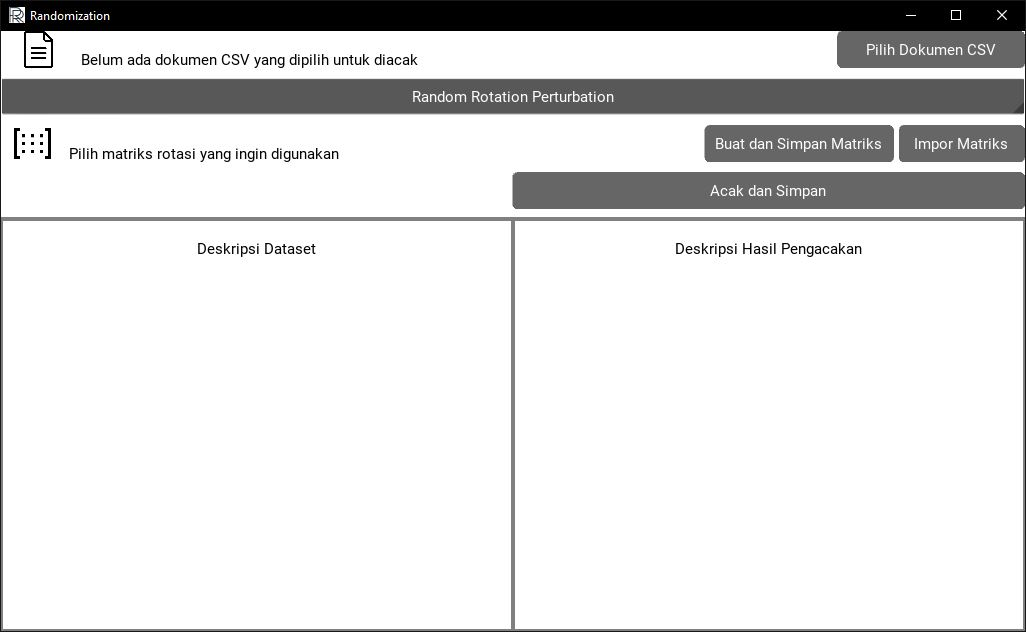
\includegraphics[scale=0.6]{antarmukautama}
	\caption{Tampilan perangkat lunak yang pertama ditampilkan saat perangkat lunak baru dibuka}
	\label{fig:antarmukautama}
\end{figure}

Antarmuka perangkat lunak mempunyai tiga buah bagian yang mempunyai fungsinya masing-masing. Ketiga bagian ini dapat dilihat pada Gambar~\ref{fig:antarmukautamabernomor} Pertama adalah bagian masukan dan pengaturan, terdapat pada bagian atas yang bernomor satu dan dikelilingi kotak merah. Kedua adalah bagian deskripsi dataset, terdapat pada bagian bawah sebelah kiri yang bernomor dua dan dikelilingi kotak biru. Terakhir adalah bagian deskripsi hasil randomisasi, terdapat pada bagian bawah sebelah kanan yang bernomor tiga dan dikelilingi kotak hijau. Ketiga bagian ini akan dijelaskan secara rinci pada subbab-subbab berikutnya.

\begin{figure}
	\centering
	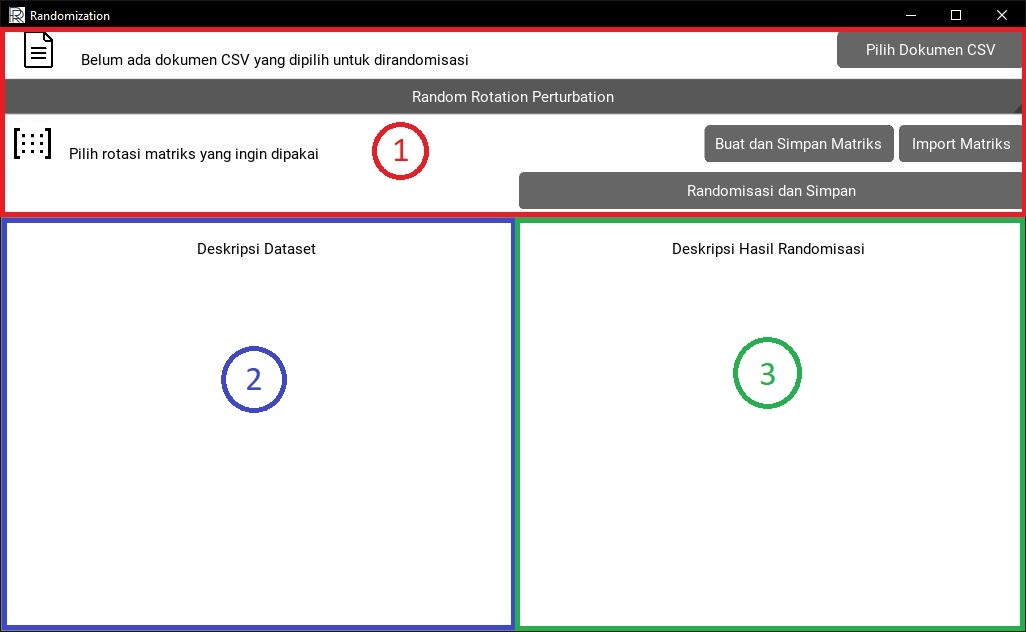
\includegraphics[scale=0.6]{antarmukautamabernomor}
	\caption{Bagian-bagian pada antarmuka perangkat lunak}
	\label{fig:antarmukautamabernomor}
\end{figure}

Perangkat lunak randomisasi ini mengimplementasikan dua buah teknik randomisasi yang berbeda yaitu \textit{Random Rotation Perturbation} dan \textit{Random Projection Perturbation}. Oleh karena itu, antarmuka perangkat lunak akan menyesuaikan dengan teknik yang dipilih oleh pengguna. Ketiga bagian antarmuka yang telah disebutkan tadi dengan otomatis akan berubah sesuai dengan teknik yang dipilih. Pada setiap subbab akan dijelaskan juga sekaligus perbedaan antarmuka teknik randomisasi satu dengan yang lainnya.

\subsection{Masukan dan Pengaturan}
\label{sec:masukanpengaturan}

Bagian masukan dan pengaturan menyediakan berbagai interaksi untuk pengguna dapat mengatur masukan yang perlu diberikan kepada perangkat lunak dan menerapkan teknik randomisasi yang diinginkan. Ada beberapa fungsi inti pada bagian ini yaitu masukan dataset berupa file \textit{comma-separated values} yang ingin dirandomisasi, memilih teknik randomisasi yang ingin digunakan, membuat baru dan memilih matriks rotasi atau proyeksi yang ingin digunakan, masukan nilai variabel Epsilon dan nilai variabel K untuk teknik \textit{Random Projection Perturbation}, dan sebuah tombol untuk menerapkan teknik randomisasi dan menyimpan hasilnya. Berikut akan dijelaskan secara rinci dengan gambar setiap fungsi tersebut yang dapat dilihat pada Gambar~\ref{fig:antarmukamasukanpengaturan} dan cara pemakaiannya yang benar secara berturut. 

\begin{figure}
	\centering
	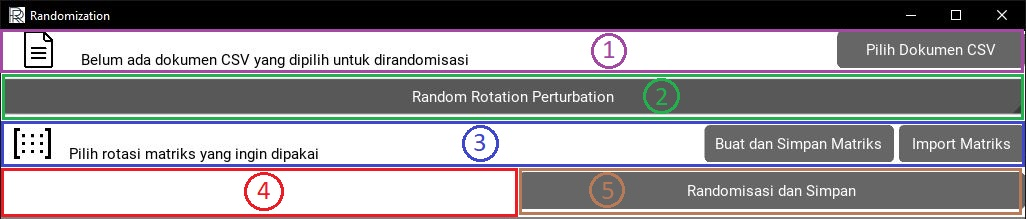
\includegraphics[scale=0.6]{antarmukamasukanpengaturan}
	\caption{Bagian antarmuka masukan dan pengaturan perangkat lunak}
	\label{fig:antarmukamasukanpengaturan}
\end{figure}

\subsubsection{Masukan Dataset}
\label{sec:masukandataset}

Pertama pengguna perlu memberikan masukan dataset yang ingin dirandomisasi berupa dokumen berjenis \textit{comma-separated values}. Perangkat lunak menyediakan fitur tersebut yang dapat dilihat pada Gambar~\ref{fig:antarmukamasukanpengaturan} yang terdapat pada bagian yang dikelilingi kotak berwarna merah dan bernomor satu. Pengguna dapat menekan tombol "Pilih Dokumen CSV" yang terletak pada ujung sebelah kanan. Tombol ini bertujuan untuk memilih dokumen yang ingin dirandomisasi pada direktori pengguna. Ketika tombol ditekan, perangkat lunak akan membuka jendela baru untuk memilih dokumen yang dapat dilihat pada gambar~\ref{fig:pilihdokumen}.

\begin{figure}
	\centering
	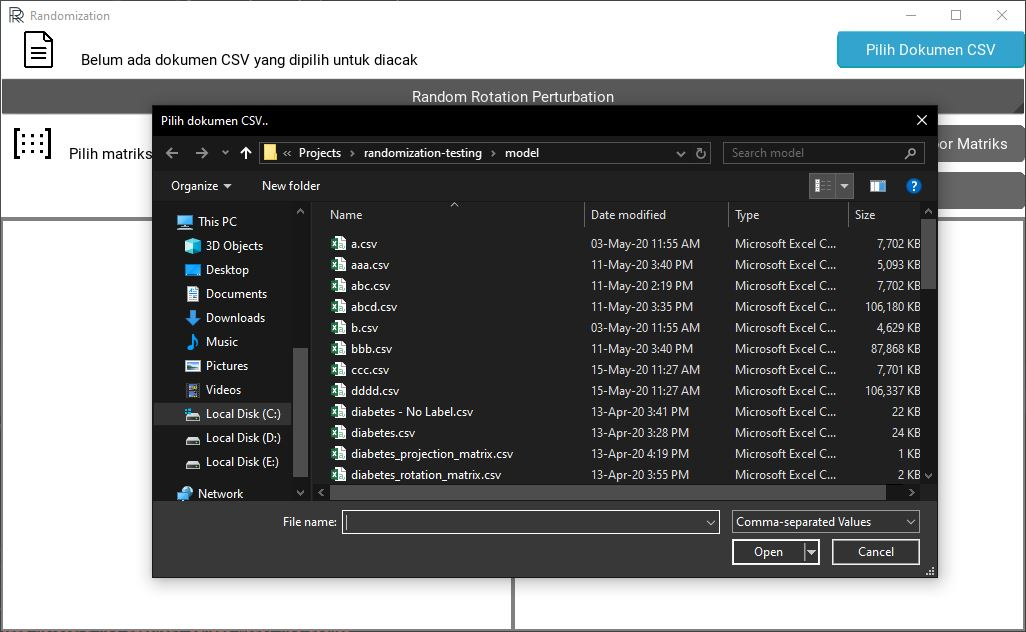
\includegraphics[scale=0.6]{pilihdokumen}
	\caption{Jendela untuk memilih dataset yang berupa dokumen CSV}
	\label{fig:pilihdokumen}
\end{figure}

Setelah pengguna memilih dataset yang diinginkan, perangkat lunak akan otomatis menuliskan lokasi dokumen yang dipilih berada. Perangkat lunak akan menampilkan lokasi dokumen tersebut pada bagian tengah sebelah kanan simbol dokumen dan sebelah kiri tombol "Pilih Dokumen CSV". Jika belum ada dataset yang dipilih maka perangkat lunak akan menampilkan label yang berupa kalimat "Belum ada dokumen CSV yang dipilih untuk dirandomisasi" yang menunjukkan bahwa belum ada dokumen yang dipilih oleh pengguna. Jika pengguna memilih ulang dokumen, maka secara otomatis juga perangkat lunak akan memperbaharui lokasi dokumen sesuai dokumen yang dipilih pengguna.

Apabila dokumen yang dipilih berukuran besar, maka perangkat lunak akan memakan sedikit waktu yang lebih lama. Dalam rangka memberitahukan kepada pengguna bahwa perangkat lunak sedang melakukan proses pemilihan dokumen, perangkat lunak akan menampilkan sebuah \textit{popup} yang memberitahukan bahwa proses pemilihan sedang berjalan dan perangkat lunak tidak berhenti bekerja maupun \textit{error} sehingga pengguna tidak bingung apabila perangkat lunak memakan waktu yang lebih lama untuk memproses dokumen yang dipilih. Tampilan antarmuka \textit{popup} tersebut dapat dilihat pada Gambar~\ref{fig:loadingmemilihdokumen}. Setelah dokumen dipilih pengguna dan perangkat lunak berhasil memproses dokumen tersebut, perangkat lunak akan memperbaharui lokasi dokumen dan menampilkan beberapa informasi dataset yang dipilih pada bagian deskripsi dataset yang akan dijelaskan pada subbab berikutnya. Tampilan antarmuka setelah pengguna memilih dokumen dapat dilihat pada Gambar~\ref{fig:dokumendipilih}

\begin{figure}
	\centering
	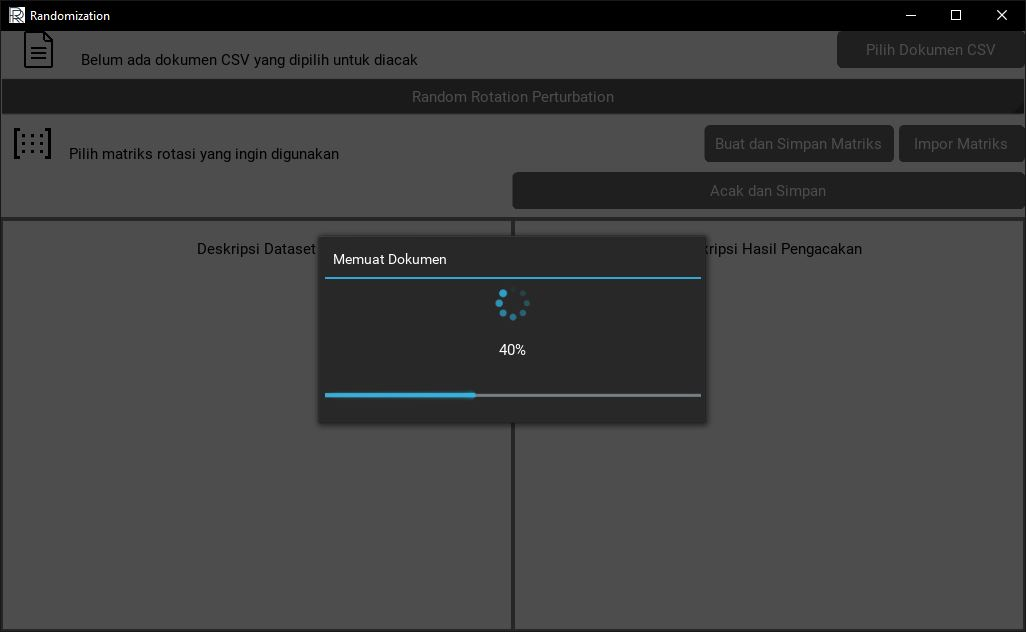
\includegraphics[scale=0.6]{loadingmemilihdokumen}
	\caption{Tampilan \textit{popup} yang ditampilkan saat proses berlangsung}
	\label{fig:loadingmemilihdokumen}
\end{figure}

\begin{figure}
	\centering
	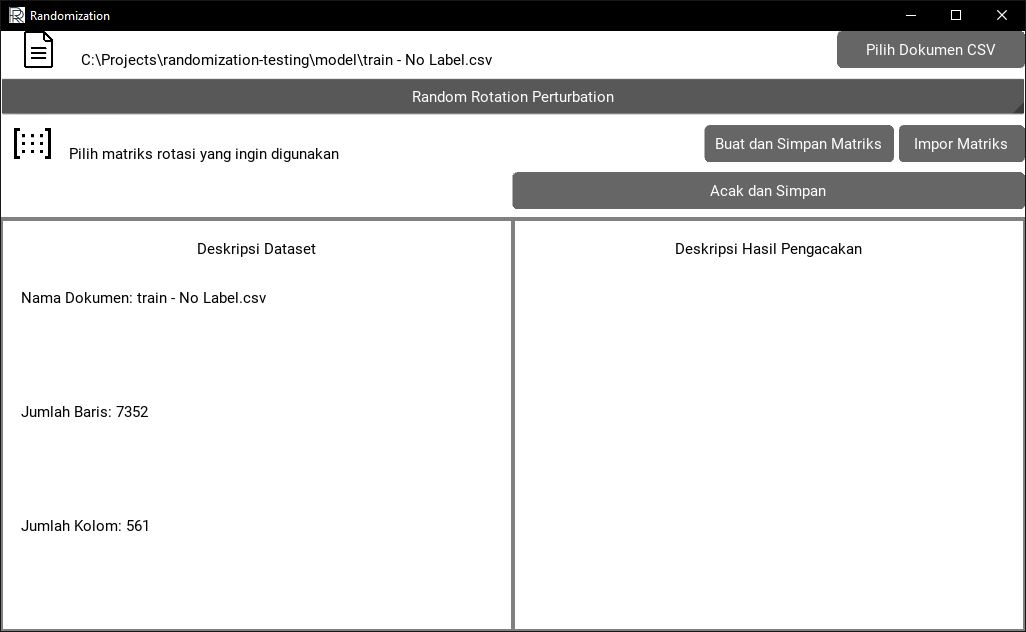
\includegraphics[scale=0.6]{dokumendipilih}
	\caption{Tampilan antarmuka setelah sebuah dokumen dipilih}
	\label{fig:dokumendipilih}
\end{figure}

Selain itu setelah pengguna memilih dokumen CSV, perangkat lunak akan membaca dokumen tersebut dan memproses isi dari dokumen tersebut menjadi dataset yang berupa matriks. Proses ini dilakukan sekali saja tepat setelah pengguna memilih dokumen dengan menekan tombol "Pilih Dokumen CSV". Oleh karena itu, apabila sebuah dokumen CSV diubah isinya setelah dokumen tersebut dipilih oleh pengguna maka perangkat lunak tetap akan menggunakan isi dari dokumen tersebut yang belum diubah. Pengguna harus berhati-hati apabila isi dokumen diubah maka pengguna juga harus memilih kembali dokumen yang sama tersebut walaupun perangkat lunak sudah menunjukkan lokasi dokumen yang digunakan adalah dokumen yang pengguna inginkan.

\subsubsection{Pemilihan Teknik Randomisasi}
\label{sec:pilihteknik}

Setelah pengguna memilih dataset yang ingin dirandomisasi, pengguna juga harus memilih teknik randomisasi apa yang ingin diterapkan terhadap dataset yang sudah dipilih. Pada awal perangkat lunak dibuka, secara otomatis teknik \textit{Random Rotation Perturbation} yang dipilih. Apabila pengguna ingin mengganti teknik yang ingin diterapkan pada dataset, pengguna dapat menekan tombol \textit{dropdown} yang bertuliskan nama teknik randomisasi. Tombol ini dapat dilihat pada Gambar~\ref{fig:antarmukamasukanpengaturan} yang dikelilingi kotak berwarna hijau dan bernomor dua.

Apabila pengguna menekan tombol ini maka perangkat lunak akan menampilkan \textit{dropdown} yang mempunyai dua buah opsi teknik randomisasi yaitu "Random Rotation Perturbation" dan "Random Projection Perturbation". Antarmuka tersebut dapat dilihat pada Gambar~\ref{fig:opsipilihteknik} yang dikelilingi oleh kotak merah. Pemilihan teknik ini juga akan memicu beberapa perubahan pada tampilan antarmuka perangkat lunak menyesuaikan dengan teknik yang dipilih. Beberapa perubahan pada perangkat lunak tersebut melingkupi bagian pembuatan dan pemilihan matriks, parameter teknik randomisasi, dan bagian randomisasi dan simpan yang akan dijelaskan setiap perubahan tersebut pada subbab berikutnya.

\begin{figure}
	\centering
	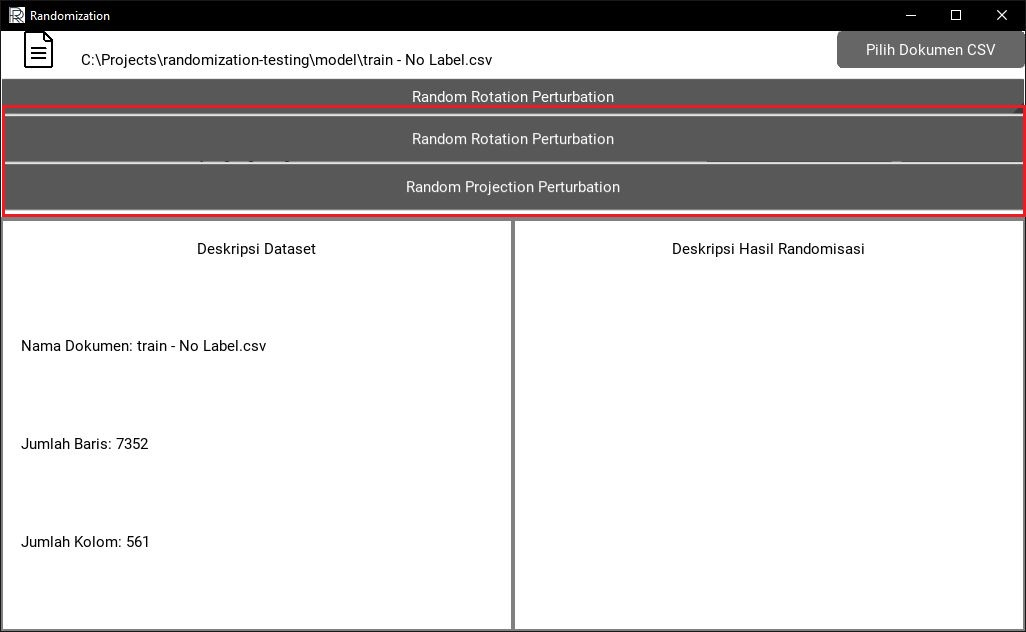
\includegraphics[scale=0.6]{opsipilihteknik}
	\caption{Tampilan antarmuka saat pengguna memilih teknik}
	\label{fig:opsipilihteknik}
\end{figure}

\subsubsection{Pembuatan dan Pemilihan Matriks}
\label{sec:pilihmatriks}

Setelah pengguna memilih teknik yang ingin diterapkan, pengguna harus memilih matriks yang diinginkan atau membuat baru. Matriks yang dimaksudkan adalah matriks rotasi atau matriks proyeksi sesuai teknik randomisasi yang dipilih. Apabila teknik \textit{Random Rotation Perturbation} yang dipilih maka perangkat lunak akan mengubah fungsi pembuatan dan pemilihan matriks ini menjadi matriks rotasi. Apabila teknik \textit{Random Projection Perturbation} yang dipilih maka perangkat lunak akan mengubah fungsi pembuatan dan pemilihan matriks ini menjadi matriks proyeksi. Perubahan ini dapat terlihat pada label yang berada di sebelah kanan simbol matriks apabila belum memilih atau membuat matriks maka label tersebut akan menampilkan kalimat "Pilih matriks rotasi yang ingin digunakan" atau "Pilih matriks proyeksi yang ingin digunakan". Bagian ini dapat dilihat pada Gambar~\ref{fig:antarmukamasukanpengaturan} yang dikelilingi oleh kotak berwarna hijau dan bernomor dua.

Ada dua buah tombol pada bagian ini yaitu "Buat dan Simpan Matriks" dan "Import Matriks". Tombol "Buat dan Simpan Matriks" mempunyai fungsi untuk membuat matriks rotasi atau proyeksi baru sesuai teknik randomisasi yang dipilih dan menyimpan matriks tersebut pada sebuah dokumen CSV baru yang dibuat oleh perangkat lunak pada direktori tertentu yang akan dipilih oleh pengguna. Pada saat perangkat lunak sedang memproses matriks tersebut, perangkat lunak akan menampilkan \textit{popup} memuat yang dapat dilihat pada Gambar~\ref{fig:buatsimpanmatriks}. \textit{Popup} ini juga akan tampil saat proses impor matriks dilakukan. Pada teknik \textit{Random Projection Perturbation}, pengguna baru bisa membuat matriks proyeksi apabila sudah memenuhi persyaratan yang diminta yaitu mengisi parameter teknik tersebut yang mana adalah variabel Epsilon dan variabel K.

Hasil matriks yang dibuat oleh perangkat lunak dapat digunakan kembali untuk lain kali sehingga rotasi atau proyeksi yang diterapkan akan sama dengan yang sebelumnya. Pengguna dapat melakukan ini dengan cara menekan tombol "Import Matriks" untuk memilih matriks rotasi atau proyeksi yang diinginkan untuk diterapkan pada dataset. Matriks yang dipilih harus sesuai dengan dataset yang ingin dirandomisasi, misalnya apabila matriks rotasi yang dipilih memiliki dimensi yang berbeda dengan dataset maka perangkat lunak akan melarang impor matriks dilakukan karena randomisasi tidak dapat dilakukan. Perangkat lunak akan menampilkan \textit{popup} peringatan untuk pengguna yang dapat dilihat pada Gambar~\ref{fig:matrikstidaksesuai}. Apabila pengguna memilih teknik \textit{Random Projection Perturbation} dan pengguna mengimpor matriks proyeksi maka parameter variabel K akan terisi secara otomatis sesuai dengan matriks proyeksi yang diimpor.

\begin{figure}
	\centering
	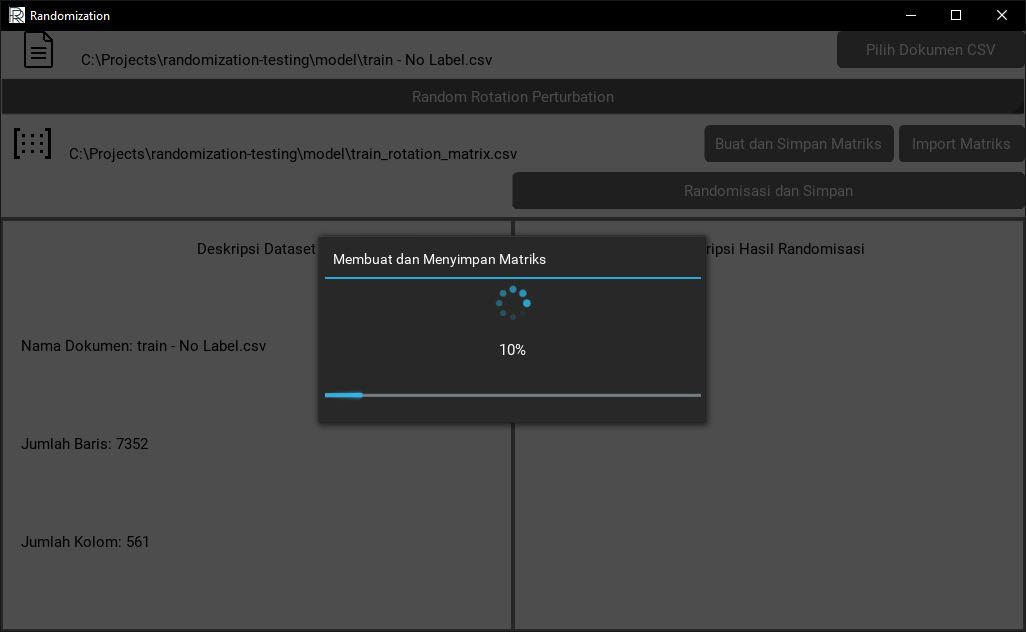
\includegraphics[scale=0.6]{buatsimpanmatriks}
	\caption{Tampilan antarmuka saat perangkat lunak membuat dan menyimpan matriks}
	\label{fig:buatsimpanmatriks}
\end{figure}

\begin{figure}
	\centering
	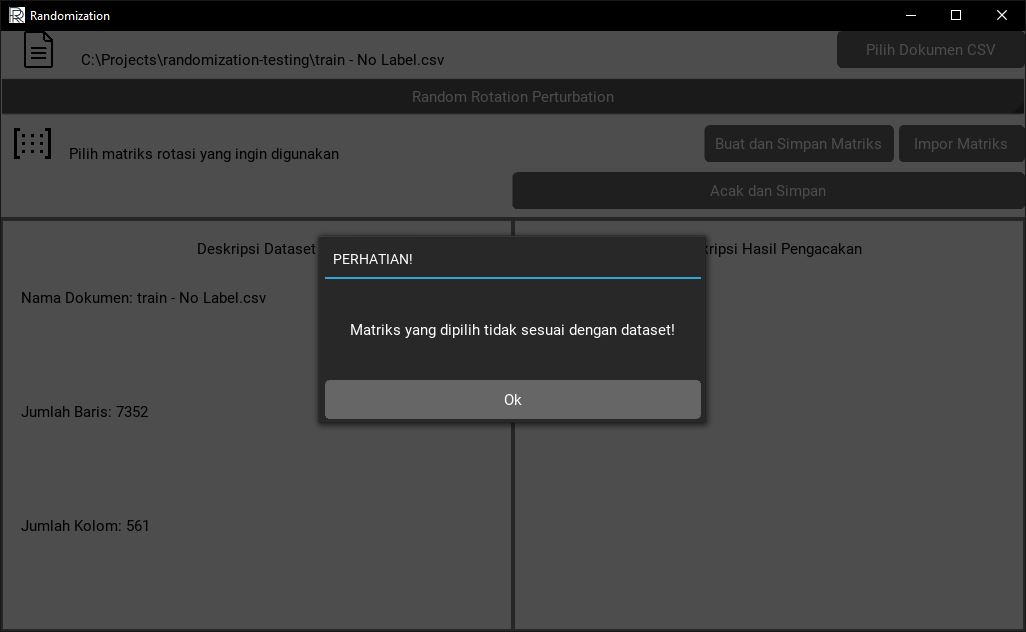
\includegraphics[scale=0.6]{matrikstidaksesuai}
	\caption{Tampilan \textit{popup} yang ditampilkan apabila matriks yang ingin diimpor tidak sesuai dengan dataset}
	\label{fig:matrikstidaksesuai}
\end{figure}

Apabila pengguna belum memilih dataset yang ingin dirandomisasi, pengguna tidak dapat membuat maupun impor matriks terlebih dahulu. Hal ini dikarenakan perlu ada proses pengecekan terlebih dahulu yang dilakukan perangkat lunak untuk memastikan dataset yang ingin dirandomisasi sudah sesuai persyaratan dan sesuai dengan matriks yang akan dipilih. Perangkat lunak akan melarang pengguna membuat maupun impor matriks dengan menampilkan sebuah \textit{popup} peringatan yang dapat dilihat pada Gambar~\ref{fig:larangmatriks}

\begin{figure}
	\centering
	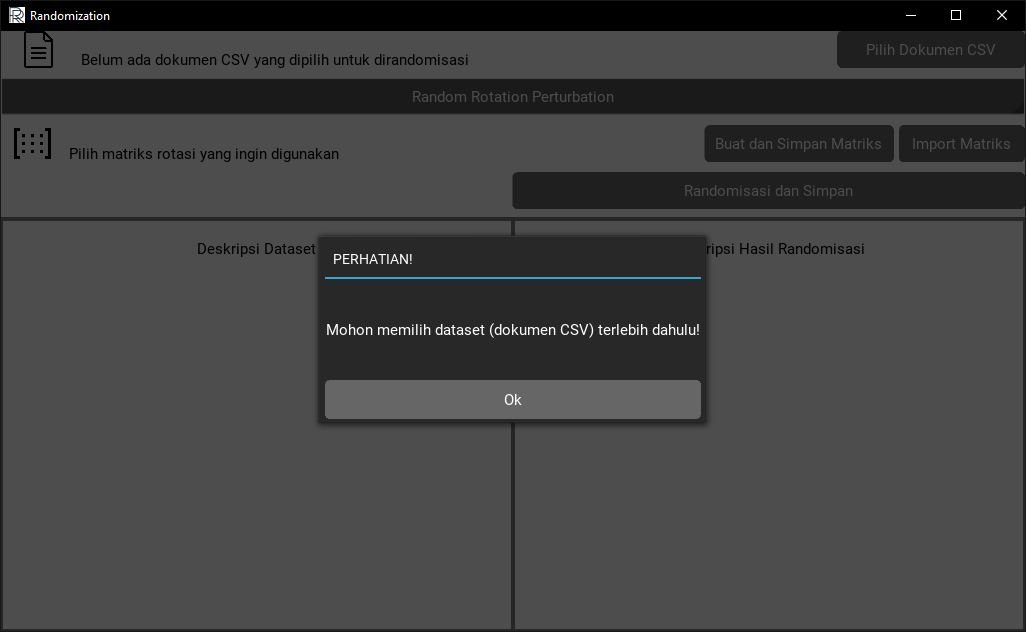
\includegraphics[scale=0.6]{larangmatriks}
	\caption{Tampilan \textit{popup} yang ditampilkan apabila pengguna belum memilih dataset yang ingin dirandomisasi}
	\label{fig:larangmatriks}
\end{figure}

\subsubsection{Parameter Teknik Randomisasi}
\label{sec:parameterteknik}

Perangkat lunak hanya meminta kepada pengguna parameter untuk teknik \textit{Random Projection Perturbation} saja apabila pengguna memilih teknik tersebut. Pada teknik \textit{Random Rotation Perturbation} tidak ada parameter yang perlu pengguna berikan. Ada dua buah parameter yang perlu pengguna berikan yaitu variabel Epsilon dan variabel K. Pengguna dapat memasukkan nilai kedua variabel tersebut dengan menekan kolom variabel tersebut masing-masing. Kedua buah parameter tersebut dapat dilihat antarmukanya pada Gambar~\ref{fig:parameterprojection}

\begin{figure}
	\centering
	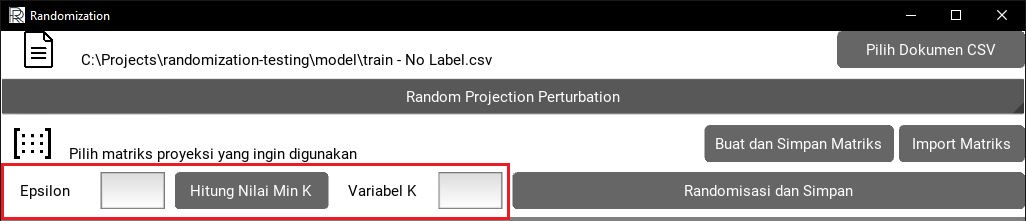
\includegraphics[scale=0.6]{parameterprojection}
	\caption{Tampilan antarmuka parameter teknik randomisasi \textit{Random Projection Perturbation}}
	\label{fig:parameterprojection}
\end{figure}

Seperti yang disinggung pada subbab sebelumnya antarmuka perangkat lunak akan menyesuaikan secara otomatis sesuai teknik yang dipilih pengguna. Pada bagian parameter teknik randomisasi, perangkat lunak akan menyembunyikan antarmuka parameter \textit{Random Projection Perturbation} apabila pengguna memilih teknik \textit{Random Rotation Perturbation}. Antarmuka tersebut dapat dilihat pada Gambar~\ref{fig:antarmukamasukanpengaturan} yang dikelilingi oleh kotak berwarna merah dan bernomor empat, dapat dilihat tidak ada parameter apapun yang tampil apabila teknik \textit{Random Rotation Perturbation} yang dipilih.

Selain dua buah parameter, pada bagian ini juga ada sebuah tombol yaitu "Hitung Nilai Min K" yang memiliki fungsi untuk menghitung nilai minimal variabel K yang pengguna berikan. Pada teknik \textit{Random Projection Perturbation}, ada beberapa persyaratan yang harus dipenuhi oleh pengguna dan salah satunya adalah variabel K yang diberikan harus melebihi sebuah nilai minimal yang dihitung berdasarkan ukuran dataset dan nilai variabel Epsilon. Oleh karena itu, sebelum tombol ini dapat berfungsi, pengguna harus memilih terlebih dahulu dataset yang ingin dirandomisasi dan memberikan masukan nilai variabel Epsilon. Apabila pengguna belum memenuhi kedua persyaratan tersebut, tombol tidak akan berfungsi dan perangkat lunak akan menampilkan \textit{popup} peringatan yang dapat dilihat pada Gambar~\ref{fig:popuphitungk}. Nilai minimal variabel K akan ditampilkan pada bagian antarmuka deskripsi dataset yang akan dijelaskan pada subbab berikutnya.

\begin{figure}
	\centering
	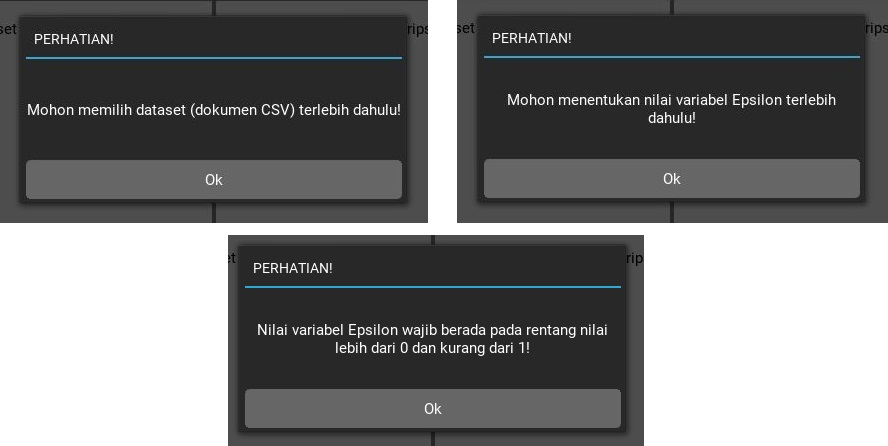
\includegraphics[scale=0.6]{popuphitungk}
	\caption{Tampilan \textit{popup} peringatan tombol "Hitung Nilai Min K"}
	\label{fig:popuphitungk}
\end{figure}

Perangkat lunak juga akan memberikan peringatan apabila nilai minimal K melebihi dimensi dari dataset yang ingin dirandomisasi karena salah satu persyaratan dari teknik \textit{Random Projection Perturbation} adalah nilai variabel K harus lebih kecil daripada jumlah dimensi pada dataset yang ingin dirandomisasi. Apabila pengguna melakukan impor matriks maka variabel K akan terisi secara otomatis dan pengguna harus menyesuaikan nilai variabel Epsilon dengan variabel K yang tidak boleh diubah oleh pengguna. 

\subsubsection{Randomisasi dan Simpan}
\label{sec:randomisasisimpan}

Setelah pengguna memberikan masukan yang sesuai dan mengatur pengaturan yang diinginkan maka pengguna telah dapat melakukan randomisasi dengan menekan tombol "Randomisasi dan Simpan". Tombol ini akan menerapkan teknik randomisasi yang dipilih oleh pengguna terhadap dataset yang ingin dirandomisasi menggunakan matriks yang telah dibuat atau dipilih oleh pengguna dan parameter-parameter yang pengguna berikan. Tampilan antarmuka saat proses randomisasi dilakukan perangkat lunak dapat dilihat pada Gambar~\ref{fig:loadingrandomisasi}.

\begin{figure}
	\centering
	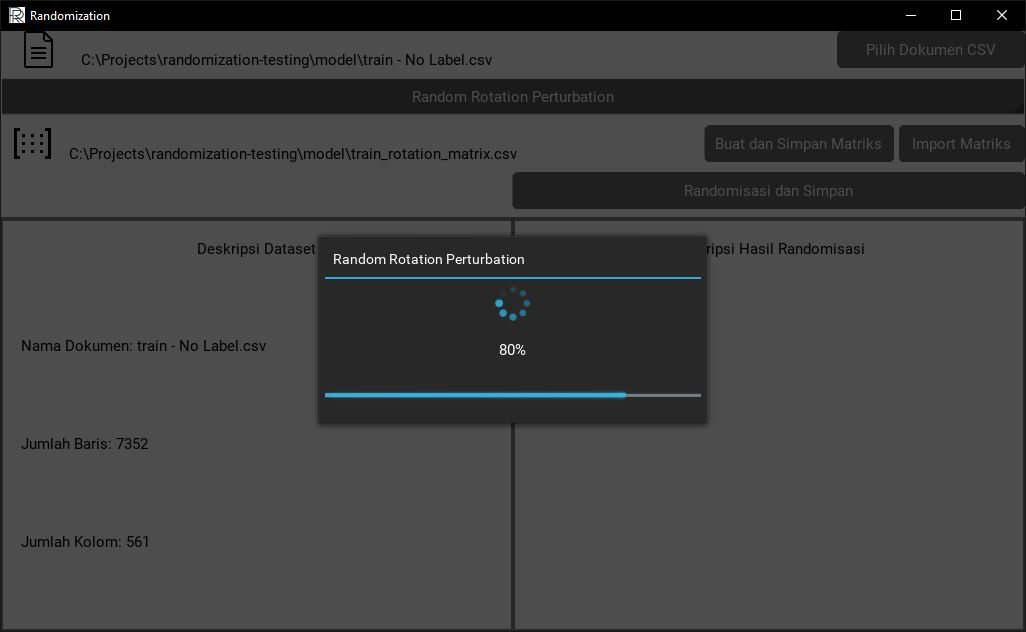
\includegraphics[scale=0.6]{loadingrandomisasi}
	\caption{Tampilan saat perangkat lunak sedang melakukan proses randomisasi}
	\label{fig:loadingrandomisasi}
\end{figure}

Setelah perangkat lunak berhasil melakukan randomisasi, perangkat lunak akan meminta pengguna untuk memilih direktori tempat penyimpanan dan nama dokumen hasil randomisasi. Perangkat lunak akan menyimpan hasil randomisasi dalam bentuk dokumen berjenis \textit{comma-separated values}. Jendela baru untuk memilih direktori penyimpanan akan ditampilkan perangkat lunak, apabila pengguna membatalkan atau dengan kata lain menutup jendela tersebut tanpa memilih direktori penyimpanan maka perangkat lunak tidak akan melanjutkan proses randomisasi dan dianggap gagal. Tampilan antarmuka \textit{popup} yang akan tampil setelah perangkat lunak berhasil melakukan proses randomisasi dan menyimpan hasilnya pada direktori yang pengguna pilih dapat dilihat pada Gambar~\ref{fig:popupberhasilrandomisasi}. Perangkat lunak juga akan menampilkan berbagai informasi hasil randomisasi pada bagian antarmuka deskripsi hasil randomisasi yang akan dijelaskan pada subbab berikutnya.

\begin{figure}
	\centering
	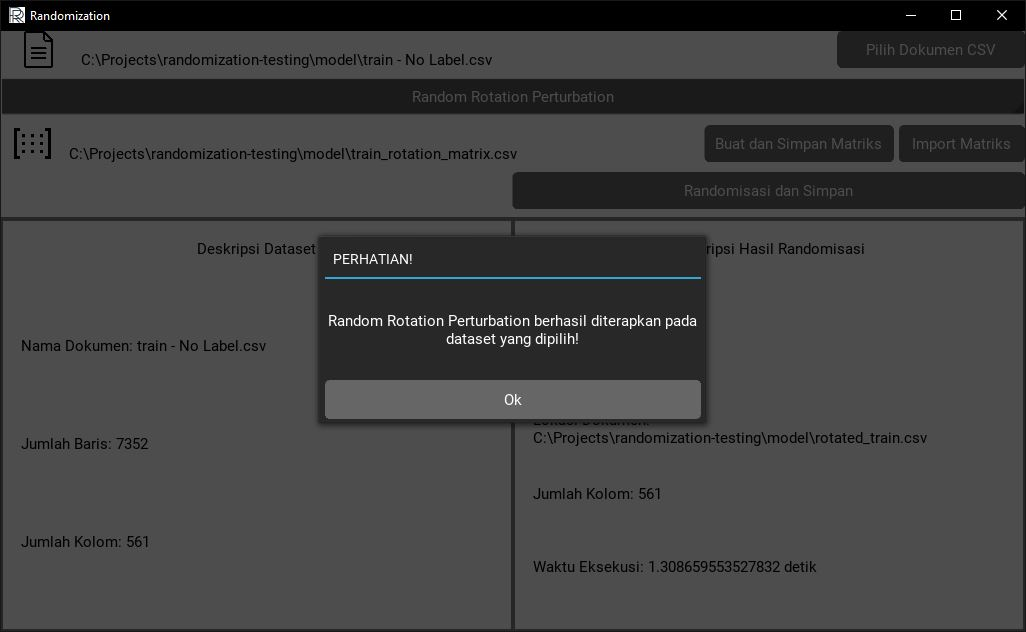
\includegraphics[scale=0.6]{popupberhasilrandomisasi}
	\caption{Tampilan \textit{popup} untuk memberitahukan pengguna bahwa randomisasi berhasil dilakukan}
	\label{fig:popupberhasilrandomisasi}
\end{figure}

Ada beberapa persyaratan yang harus dipenuhi oleh penggun sebelum melakukan randomisasi yaitu memilih dataset yang ingin dirandomisasi, memilih teknik randomisasi yang diinginkan, membuat atau memilih matriks rotasi atau proyeksi, dan memberikan masukan nilai yang sesuai persyaratan yang ada kepada parameter-parameter teknik randomisasi. Apabila ada persyaratan yang tidak dipenuhi oleh pengguna maka perangkat lunak akan menampilkan \textit{popup} untuk memberikan peringatan kepada pengguna dan perangkat lunak tidak akan melanjutkan proses randomisasi. Perangkat lunak akan menampilkan \textit{popup} peringatan terhadap pelanggaran masing-masing persyaratan tersebut yang dapat dilihat pada Gambar~\ref{fig:}

\begin{figure}
	\centering
	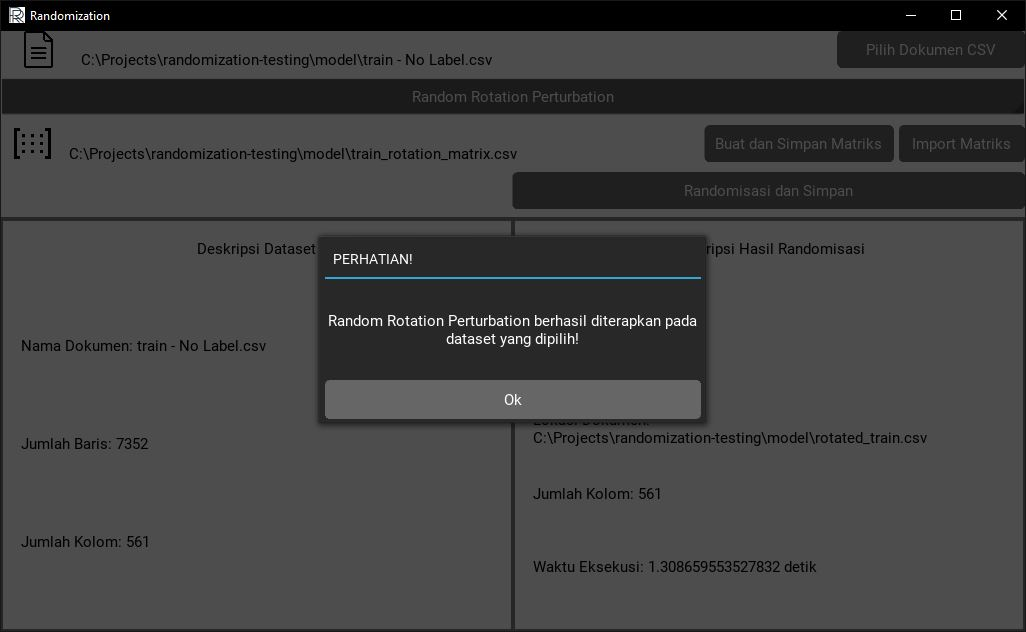
\includegraphics[scale=0.6]{popupberhasilrandomisasi}
	\caption{Tampilan \textit{popup} untuk memberitahukan pengguna bahwa randomisasi berhasil dilakukan}
	\label{fig:popupberhasilrandomisasi}
\end{figure}



\subsection{Deskripsi Dataset}
\label{sec:deskripsidataset}

\subsection{Deskripsi Hasil Randomisasi}
\label{sec:masukanpengaturan}



\section{Pengujian Perangkat Lunak}
\label{sec:pengujianpl}

\subsection{Pengujian Fungsional}
\label{sec:pengujianfungsional}

\subsection{Pengujian Eksperimental}
\label{sec:pengujianeksperimental}